\documentclass[11pt]{article}

\usepackage[margin=1in]{geometry}
\usepackage{amsmath,amssymb,amsthm}
\usepackage{enumitem}
\usepackage{graphicx}
\usepackage[hidelinks]{hyperref}

\newtheorem{theorem}{Theorem}
\newtheorem{corollary}{Corollary}

\newcommand{\ccc}{\mathrm{c.c.c.}}
\newcommand{\cf}{\operatorname{cf}}
\newcommand{\dens}{\operatorname{dens}}
\newcommand{\fin}{\mathrm{fin}}
\newcommand{\R}{\mathbb{R}}
\newcommand{\N}{\mathbb{N}}
\newcommand{\D}{\mathcal{D}}
\newcommand{\F}{\mathcal{F}}
\newcommand{\B}{\mathcal{B}}
\newcommand{\CI}{C_I}
\newcommand{\GCH}{\mathsf{GCH}}
\newcommand{\ZFC}{\mathsf{ZFC}}
\newcommand{\DiamondE}{\Diamond(E^\kappa_\omega)}

\title{A Conditional Weakening of GCH in the Koszmider--Shelah--Swietek Construction}
\author{arXiv automatic math run \texttt{fa\_banach\_001}}
\date{Candidate conditional packet, June 14, 2026}

\begin{document}
\maketitle

\section*{Classification}

\begin{itemize}[leftmargin=2em]
\item \textbf{Status:} conditional reduction.
\item \textbf{Source:} P. Koszmider, S. Shelah, M. Swietek,
\emph{There is no bound on sizes of indecomposable Banach spaces},
arXiv:1603.01753; Adv. Math. 323 (2018), 745--783.
\item \textbf{Target:} the Introduction asks whether the generalized
continuum hypothesis can be removed from Theorem 1.3, which under \(\GCH\)
produces, above every cardinal, an indecomposable \(C(K)\)-space with few
operators.
\end{itemize}

\section*{Source Question}

On page 5, immediately after the repeated Theorem 5.3, the source paper asks
whether the \(\GCH\) hypothesis can be removed from Theorem 1.3.  In the
parsed source, this is line 396 of \texttt{source.tex}.

\begin{center}
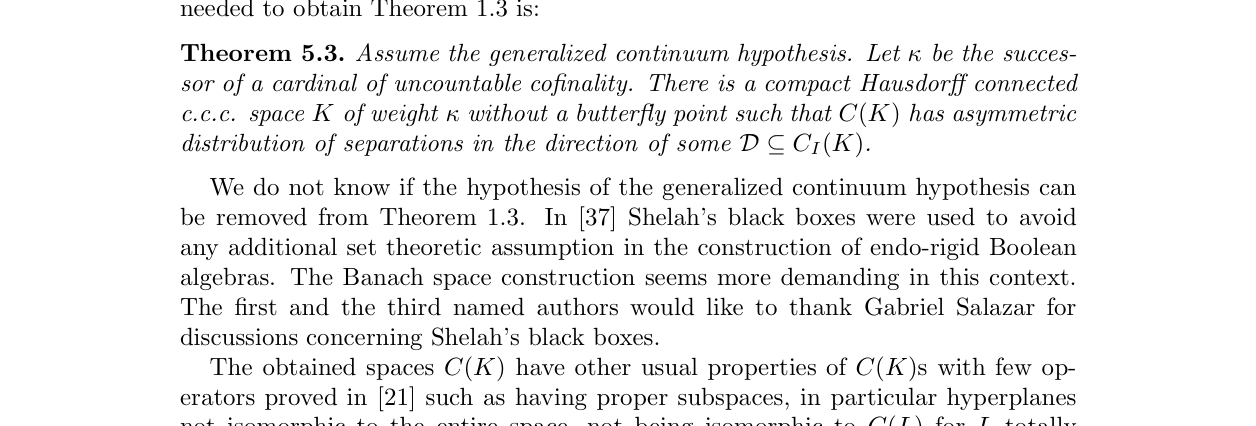
\includegraphics[width=\linewidth]{figures/open_problem_page5_gch_removal.png}
\end{center}

\section*{Conditional Dependencies}

This packet does \emph{not} prove the full \(\ZFC\) version of the source
question.  It isolates two assumptions which are sufficient for the source
construction at a fixed cardinal.

Let \(\kappa\) be a regular cardinal which is the successor of a cardinal of
uncountable cofinality.  The dependencies are:
\begin{enumerate}[label=(\(\mathrm{H}\arabic*\)), leftmargin=3em]
\item \(\kappa^\omega=\kappa\) and \(\alpha^\omega<\kappa\) for every
\(\alpha<\kappa\).
\item \(\DiamondE\): there is a sequence
\((S_\alpha)_{\alpha\in E^\kappa_\omega}\) such that \(S_\alpha\subseteq
\alpha\) and, for every \(X\subseteq\kappa\), the set
\[
\{\alpha\in E^\kappa_\omega: X\cap\alpha=S_\alpha\}
\]
is stationary in \(\kappa\).
\end{enumerate}

Under \(\GCH\), the source obtains (H1) from Lemma 5.1 and (H2) from
Gregory's theorem, quoted as Theorem 5.2.  The point of the packet is that the
rest of the argument uses only these two consequences.

\section*{Proof Intuition}

The source proof uses \(\GCH\) as infrastructure, not as a Banach-space
ingredient.  Countable cardinal arithmetic keeps the Boolean completion, the
function families, and the possible countable codes at size \(\kappa\), and
also makes the coding-closure set club.  The diamond sequence then guesses the
eventual countable data needed at stationarily many stages of the ladder
recursion.  Once these two ingredients are assumed directly, every later
topological and operator-theoretic step is exactly the source argument:
construct the ladder family, obtain asymmetric distribution of separations,
deduce few-star operators from the c.c.c. space, upgrade to few operators
using absence of butterfly points, and conclude indecomposability from
connectedness.

\section*{Conditional Theorem}

\begin{theorem}
Let \(\kappa\) be a regular cardinal which is the successor of a cardinal of
uncountable cofinality.  Assume (H1) and (H2) above.  Then there is a compact
Hausdorff connected \(\ccc\) space \(K\) of weight \(\kappa\), without a
butterfly point, such that \(C(K)\) has asymmetric distribution of separations
in the direction of some \(\D\subseteq \CI(K)\).  Consequently, \(C(K)\) has
few operators and is indecomposable, and \(\dens C(K)=\kappa\).
\end{theorem}

\begin{proof}
We verify that the proof of Theorem 5.3 of the source paper works with (H1)
and (H2) in place of \(\GCH\).

First, the source Lemma 3.13, labelled ``GCH'' in the paper, proves that
\(\dens C(\nabla\F)=\kappa\) for the relevant
\(\D\subseteq\F\subseteq \CI(L)\).  Inspecting its proof, the only cardinal
calculation is that the completed free Boolean algebra \(\overline{Fr}(\kappa)\)
has cardinal at most \(\kappa^\omega\), because every element is the supremum
of a countable subset of the free algebra \(Fr(\kappa)\).  Thus the proof
needs only \(\kappa^\omega=\kappa\), which is part of (H1).  The lower bound
comes from the coordinate family \(\D\), and the upper bound comes from the
Stone-Weierstrass estimate inside \(C(L)\), as in the source proof.

Second, at the beginning of Section 5, the source Lemma 5.1 is used only for
the two displayed conclusions
\[
\kappa^\omega=\kappa
\quad\text{and}\quad
\alpha^\omega<\kappa\quad(\alpha<\kappa).
\]
These are exactly (H1).  They give the size of the coding space
\[
(\{-2,-1\}\cup\kappa)\times\{-1,1\}^{\N}\times
\bigl(\CI(L)^{\N}\cup\B(\CI(L))^{\N}\bigr)
\]
as \(\kappa\), so the bijection \(\Psi\) used by the construction exists.
They also supply the standard closure argument showing that the set \(C_\Psi\)
of ordinals closed under the coding map is club in \(\kappa\).

Third, the only use of source Theorem 5.2 is to obtain a
\(\DiamondE\)-sequence.  This is exactly (H2).  With that sequence fixed, the
recursive definition of the ladder family \(\F\) is verbatim the construction
in Theorem 5.3.  At a stage \(\gamma<\kappa\), the existence of the required
\(\alpha_\gamma\in E^\kappa_\omega\cap C_\Psi\) follows from (H2), because
the target code \(X\subseteq\kappa\) is guessed on a stationary set and
\(C_\Psi\) is club.  The rest of the stage uses only the source lemmas on
ladder families, countable separating subfamilies, and nonseparation along an
infinite \(M\subseteq\N\).

The verification of asymmetric distribution of separations is also unchanged.
Given pairwise disjoint \((f_n)\), antichains \((U_n)\), signs
\((\nu^\xi_n)\), and refinements \((U^\xi_n)\), code all of this by a subset
of \(\kappa\).  By (H2) choose a guessed \(\alpha\in E^\kappa_\omega\cap
C_\Psi\) above a bound \(\beta\) containing the supports of the data.  The
ladder family stage at \(\alpha\) supplies
\[
g_\alpha=\bigvee_{n\in M_\alpha}
\bigl(f_n d_{\eta^\alpha_n,\nu^{\eta^\alpha_n}_n}\bigr)
\]
and the nonseparation conclusion required in Definition 1.5 of the source
paper.  Thus \(C(\nabla\F)\) has asymmetric distribution of separations in the
direction of \(\{d_\alpha:\alpha<\kappa\}\).

The source lemmas on ladder families then give that \(K=\nabla\F\) is
connected and has no butterfly point; the source c.c.c. argument for
\(L_\kappa\) and its continuous image gives that \(K\) is \(\ccc\); and the
density computation above gives weight and density \(\kappa\).  Applying
source Theorem 2.1 and Theorem 2.4, asymmetric distribution plus \(\ccc\)
gives few-star operators, no butterfly points upgrades this to few operators,
and connectedness makes \(C(K)\) indecomposable.
\end{proof}

\begin{corollary}
If for every cardinal \(\mu\) there is a regular successor cardinal
\(\kappa>\mu\), with predecessor of uncountable cofinality, satisfying (H1)
and (H2), then the conclusion of source Theorem 1.3 holds without assuming
full \(\GCH\): for every \(\mu\) there is an indecomposable Banach space of
density bigger than \(\mu\), of the form \(C(K)\) with few operators and
connected compact \(K\).
\end{corollary}

\begin{proof}
Apply the theorem to such a \(\kappa>\mu\).  The resulting space has density
\(\kappa\), hence density bigger than \(\mu\), and has the same few-operators
and indecomposability conclusion as in the source theorem.
\end{proof}

\section*{Verification and Novelty Notes}

The proof is a line-by-line dependency audit of the source construction, not
an independent reconstruction of the ladder family.  The critical source
locations are:
\begin{itemize}[leftmargin=2em]
\item Lemma 3.13, source lines 1116--1130, where
\(\kappa^\omega=\kappa\) is used for the density calculation.
\item Lemma 5.1, source lines 2025--2036, whose conclusions are absorbed into
(H1).
\item Theorem 5.2 and the setup before Theorem 5.3, source lines 2043--2086,
where \(\GCH\) is used to obtain \(\DiamondE\) and the coding map \(\Psi\).
\item Theorem 5.3, source lines 2088--2242, where the recursion and the final
asymmetric-distribution verification use the diamond sequence and the coding
club.
\end{itemize}

Bounded duplicate and literature checks were performed before promotion.  The
run registry, solution, attempt, and proof-gap indexes had no hit for
arXiv:1603.01753, the exact title phrase, or the GCH-removal question.  Local
corpus searches for the title/authors together with \(GCH\), diamond,
black-box, few-operator, and arbitrary-density terms did not reveal a later
exact answer.  A focused web search for the exact title and phrases such as
``GCH removed'' and ``generalized continuum hypothesis removed'' found the
source paper but no separate paper explicitly removing GCH from the arbitrary
density few-operators construction.  The result is therefore recorded only as
a candidate conditional reduction, not as a full solution of the ZFC removal
problem.

\section*{Limitations}

The packet leaves the main source question open in its full form.  In
particular, it does not prove \(\DiamondE\) in \(\ZFC\), does not prove that
the countable-coding arithmetic in (H1) holds above every cardinal, and does
not replace Shelah black boxes by a new Banach-space construction.  It only
shows that full \(\GCH\) is not used beyond the two isolated dependencies.

\section*{Human Review Recommendation}

Reviewers should first check that Lemma 3.13 has no hidden use of
\(\GCH\) beyond \(\kappa^\omega=\kappa\), and that the clubness of \(C_\Psi\)
indeed follows from \(\alpha^\omega<\kappa\) for all \(\alpha<\kappa\).
The next useful mathematical step would be either to establish (H1)+(H2) in a
weaker set-theoretic context relevant to many cardinals, or to replace
\(\DiamondE\) in the ladder recursion by a genuine black-box construction.

\begin{thebibliography}{9}

\bibitem{kss}
P. Koszmider, S. Shelah, and M. Swietek,
\emph{There is no bound on sizes of indecomposable Banach spaces},
arXiv:1603.01753; Adv. Math. 323 (2018), 745--783.

\bibitem{jech}
T. Jech,
\emph{Set Theory},
Springer Monographs in Mathematics, Springer, 2003.

\end{thebibliography}

\end{document}
